%!TEX root = ../../../adrien_gomar_phd.tex

\subsection{Convergence of the computations} % (fold)
\label{sub:dream_convergence}

\begin{figure}[htb]
  \centering
  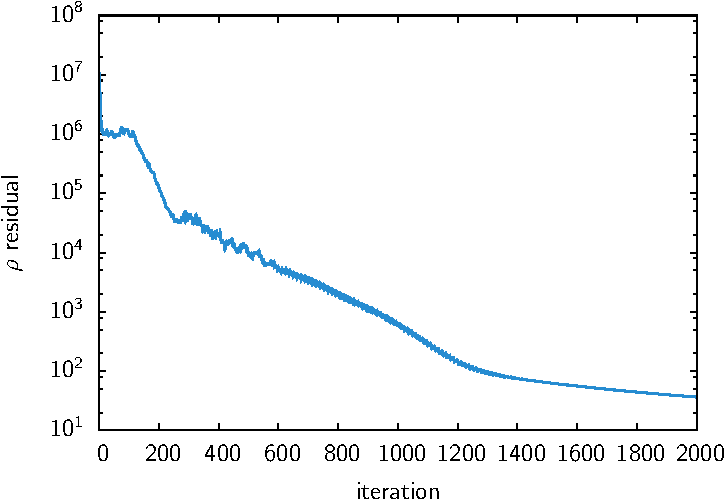
\includegraphics[width=.5\textwidth]{DREAM_LS_RESIDUALS_PPT.pdf}
  \caption{Convergence of the steady computations.}
  \label{fig:dream_operating_point}
\end{figure}

\subsection{Operating point} % (fold)
\label{sub:dream_operating_point}

\begin{table}[htb]
  \ra{1.3} \centering
  \begin{tabular}{l|ccccccccc}
    \toprule
    \phantom{abdefghijk}& $C_{t_F}$ & $C_{p_F}$ & $\eta_F$ & $C_{t_R}$ & $C_{p_R}$ & $\eta_R$ & $C_t$ & $C_p$ & $\eta$ \\
    \midrule
    Roe 1 & $0.5135$ & $0.9762$ & $0.5568$ & $0.8421$ & $1.8895$ & $0.5242$ & $1.3555$ & $2.8657$ & $0.5353$ \\
    Roe 2 & $0.5637$ & $0.9941$ & $0.6002$ & $0.8664$ & $1.8613$ & $0.5475$ & $1.4301$ & $2.8554$ & $0.5659$ \\
    Roe 3 & $0.5684$ & $0.9937$ & $0.6054$ & $0.8715$ & $1.8618$ & $0.5506$ & $1.4398$ & $2.8555$ & $0.5697$ \\
    % JST $\kappa_4 = 0.016$ & $0.6128$ & $1.0647$ & $0.6093$ & $0.9514$ & $2.0401$ & $0.5485$ & $1.5642$ & $3.1048$ & $0.5694$ \\
    JST $\kappa_4 = 0.032$ & $0.5679$ & $0.9930$ & $0.6053$ & $0.8691$ & $1.8583$ & $0.5501$ & $1.4370$ & $2.8513$ & $0.5694$ \\
    JST $\kappa_4 = 0.064$ & $0.5666$ & $0.9921$ & $0.6045$ & $0.8669$ & $1.8558$ & $0.5495$ & $1.4335$ & $2.8478$ & $0.5687$ \\
    \bottomrule
  \end{tabular}
  \caption{Flight condition parameters.}
  \label{tab:dream_operating_point}
\end{table} 

\subsection{Flow field around the blades} % (fold)
\label{sub:dream_flow_field}

\subsection{Radial profiles} % (fold)
\label{sub:dream_radial_profiles}